\documentclass[12pt,a4paper]{article}
\usepackage{extsizes}
\usepackage{geometry}
\geometry{a4paper, margin=1.0in}


\usepackage[table, svgnames, dvipsnames]{xcolor}
\usepackage{color}

\usepackage{float}
\usepackage{graphicx, subfigure}
\usepackage{pdfpages}
\usepackage[multidot]{grffile}

\usepackage{siunitx}
\usepackage{listings}
\usepackage{tcolorbox}
\tcbuselibrary{breakable}
\tcbuselibrary{skins}
\tcbuselibrary{listings}

\definecolor{dkgreen}{rgb}{0,0.6,0}
\definecolor{gray}{rgb}{0.5,0.5,0.5}
\definecolor{lightgray}{rgb}{0.8,0.8,0.8}
\definecolor{mauve}{rgb}{0.58,0,0.82}

\lstset{frame=tBLr,
	%	frameround=fttt,
	language=Matlab,
	aboveskip=3mm,
	belowskip=3mm,
	showstringspaces=false,
	columns=flexible,
	basicstyle={\small\ttfamily},
	lineskip=0.5em,
	xleftmargin=23pt,
	xrightmargin=9pt,
	framexleftmargin=17pt,
	framexrightmargin=5pt,
	framexbottommargin=2pt,
	numbers=left,
	firstnumber=1,
	numberstyle=\tiny\color{gray},
	keywordstyle=\color{blue},
	commentstyle=\color{dkgreen},
	stringstyle=\color{mauve},
	rulecolor=\color{black},
	breaklines=true,
	breakatwhitespace=true,
	tabsize=4,
}



\definecolor{shadecolor}{gray}{0.95}
\definecolor{captionbox}{cmyk}{0.43, 0.35, 0.35,0.01}


\lstdefinelanguage{text}{
	keywords={},
}
\newtcblisting[auto counter]{wgetlisting}[2][]{%
	listing only,
	breakable,
	top=0.5pt,
	bottom=0.5pt,
	colback=red!5!white,
	colframe=red!25,
	left=6mm,
	sharp corners,
	boxrule=0pt,
	bottomrule=1pt,
	toprule=1pt,
	enhanced jigsaw,
	listing options={%style=tcblatex,
		frame=none,
		language=text,
		xleftmargin=1pt,
		xrightmargin=1pt,
		aboveskip=0mm,
		belowskip=0mm,
		lineskip=-0.15em,
		framexbottommargin=0pt,
		%
		numbers=left,
		numberstyle=\tiny\color{red!75!black},
		moredelim={[is][keywordstyle]{@@}{@@}},
		basicstyle=\normalsize\ttfamily,
		breaklines=true,
		breakautoindent=false,
		breakindent=0pt,
		escapeinside={(*}{*)},
	},%
	lefttitle=0pt,
	coltitle=black,
	colbacktitle=white,
	title={Listing \thetcbcounter:  #2},#1%  
	borderline north={1pt}{14.4pt}{red!25,dashed},
}
% 

%https://tex.stackexchange.com/questions/476100/lstlisting-line-number-gaps
\makeatletter
\let\orig@lstnumber=\thelstnumber
\newcommand\lstsetnumber[1]{\gdef\thelstnumber{#1}}
\newcommand\lstresetnumber{\global\let\thelstnumber=\orig@lstnumber}
\newcommand\bashnumbering{\lstsetnumber{\texttt{>>}}}
\makeatother


\usepackage{setspace}
\usepackage{anyfontsize}

\setstretch{1.5}


\usepackage{amsthm, thmtools}
\usepackage{environ}
%\usepackage{bickham}
%\usepackage{boondox-cal}
%\usepackage{boondox-calo}
\usepackage{dutchcal}
\usepackage{amssymb,amsmath,gensymb,mathtools,unicode-math}
%\usepackage{pxfonts}
%\usepackage{newtxmath}
\usepackage{stackengine}


\usepackage[hyphens]{url}%\PassOptionsToPackage{hyphens}{url}
\usepackage[colorlinks,linkcolor=blue,citecolor=blue, breaklinks]{hyperref}
\usepackage{xurl}
%\usepackage{url}
%\usepackage{newtxmath}



%\usepackage{breakurl}
\usepackage{copyrightbox,doi}


\usepackage{pgffor}
\usepackage{placeins}
\usepackage{comment}
\usepackage{etoolbox}
\usepackage{longtable, ltablex, tabu}
\usepackage{tabularx,multirow,multicol,array}
\newcolumntype{C}[1]{>{\centering\arraybackslash\hspace{0pt}}p{#1}}
\newcolumntype{Y}{>{\centering\arraybackslash}X}
\definecolor{headerColor}{rgb}{0.78,0.85,.95}



\newcounter{magicrownumbers}
\newcommand\rownumber{\stepcounter{magicrownumbers}\arabic{magicrownumbers}}
\newcommand\resetrownumber{\preto\tabular{\setcounter{magicrownumbers}{0}}}
\preto\tabular{\setcounter{magicrownumbers}{0}}
\preto\longtable{\setcounter{magicrownumbers}{0}}


\usepackage{csvsimple}
\makeatletter
\csvset{
	autotabularcenter/.style={
		file=#1,
		after head=\csv@pretable\begin{tabular}{|*{\csv@columncount}{c|}}\csv@tablehead,
			table head=\hline\csvlinetotablerow\\\hline,
			late after line=\\,
			table foot=\\\hline,
			late after last line=\csv@tablefoot\end{tabular}\csv@posttable,
		command=\csvlinetotablerow},
}
\makeatother
\newcommand{\csvautotabularcenter}[2][]{\csvloop{autotabularcenter={#2},#1}}

%======================================================================================

\usepackage{fancyhdr}

\usepackage[inline]{enumitem}
\newlist{alphinline}{enumerate*}{1}
\setlist[alphinline]{label=(\alph*)}
\newlist{enuminline}{enumerate*}{1}
\setlist[enuminline]{label=(\arabic*)}
\newlist{circlelist}{enumerate}{1}
\setlist[circlelist,1]{label=\protect\circled{\arabic*}}
\newlist{alphabetlist}{enumerate}{1}
\setlist[alphabetlist]{label=\alph*)}
\newlist{checklist}{itemize}{1}
\setlist[checklist]{label=$\checkmark$)}
\newlist{iteminline}{itemize*}{1}
\setlist[iteminline]{label=$\bullet$}

\setlength\itemsep{0.7em}

\usepackage{titlesec}

\usepackage[localise=on,extrafootnotefeatures]{xepersian} %%%%%%%%%%%%%%%%%%%%%%%%%%%
\settextfont{XB Niloofar}

%\settextfont[
%Scale=1.09,
%Extension=.ttf, 
%Path=styles/fonts/,
%BoldFont=XB NiloofarBd,
%ItalicFont=XB NiloofarIt,
%BoldItalicFont=XB NiloofarBdIt
%]{XB Niloofar}

%\setdigitfont[
%Scale=1.09,
%Extension=.ttf, 
%Path=styles/fonts/,
%BoldFont=XB NiloofarBd,
%ItalicFont=XB NiloofarIt,
%BoldItalicFont=XB NiloofarBdIt
%]{XB Niloofar}
\setdigitfont{Yas}

%\defpersianfont\sayeh[
%Scale=1,
%Path=styles/fonts/
%]{XB Kayhan Pook}
%


%\makeatletter
%\def\abjad@zero{}
%\def\abj@num@i#1{%
%	\ifcase#1\or الف\or ب\or ج\or د%
%	\or ه‍\or و\or ز\or ح\or ط\fi
%	\ifnum#1=\z@\abjad@zero\fi}
%\def\abj@num@ii#1{%
%	\ifcase#1\or ی\or ک\or ل\or م\or ن%
%	\or س\or ع\or ف\or ص\fi
%	\ifnum#1=\z@\fi\abj@num@i}
%\def\abj@num@iii#1{%
%	\ifcase#1\or ق\or ر\or ش\or ت\or ث%
%	\or خ\or ذ\or ض\or ظ\fi
%	\ifnum#1=\z@\fi\abj@num@ii}
%\def\abj@num@iv#1{%
%	\ifcase#1\or غ\fi
%	\ifnum#1=\z@\fi\abj@num@iii}
%\let\@latinalph\@alph%
%\let\@latinAlph\@Alph%
%\def\PersianAlphs{%
%	\let\@alph\abjadnumeral%
%	\let\@Alph\abjadnumeral%
%}
%\def\LatinAlphs{%
%	\let\@alph\@latinalph%
%	\let\@Alph\@latinAlph%
%}
%\PersianAlphs
%\makeatother

\newcommand{\textemf}[1]{«#1»}
\titleformat{\section}{\large\bfseries}{ماده \thesection: }{0em}{}
\titleformat{\subsection}{\bfseries}{\thesubsection- }{0em}{}
\titleformat{\subsubsection}{\bfseries}{\thesubsubsection- }{0em}{}

\usepackage{bidihl}
\definecolor{lightYellow}{rgb}{1,1,0.73}
\newcommand{\hl}[1]{\bidihl{#1}}
\definecolor{bidihlcolor}{rgb}{1,1,0.73}


\AtBeginEnvironment{figure}{\setcounter{subfigure}{0}}% Resets subfigure counter at start of figure environment
%.cwl
\NewEnviron{copyrightBox}[3][b]{
	%	\setcounter{subfigure}{0}% Reset subfigure counter
	\noindent\copyrightbox[#1]{
		\begin{minipage}{#2}\BODY\end{minipage}
	}{#3}}
%.cwl
\NewEnviron{RTLcopyrightBox}[3][b]{
	%	\setcounter{subfigure}{0}% Reset subfigure counter
	\noindent\copyrightbox[#1]{
		\begin{minipage}{#2}
			\begin{RTL}	\BODY \end{RTL}
		\end{minipage}
	}{#3}}



\newcommand{\f}[2]{$\frac{#1}{#2}$}
\newcommand{\rltext}[1]{\text{\rl{#1}}}
\newcommand{\lrtext}[1]{\text{\lr{#1}}}

\newtheorem{note}{تبصره}[section]


\newcommand*{\Scale}[2][4]{\scalebox{#1}{$#2$}}%
\newcommand*{\Resize}[2]{\resizebox{#1}{!}{$#2$}}%
\newcommand\rescaleequation[2]{\resizebox{#1\hsize}{!}{$#2$}}

\usepackage{ptext}




\title{شیوه‌نامه همکاری شرکت زعیم با دانشگاه شریف و پژوهشکده شهید رضایی}
%\date{}

\begin{document}
	\pagestyle{fancy}
	
	\fancyhead[LO,RE]{صنایع الکترونیک زعیم}
	\fancyhead[C]{
	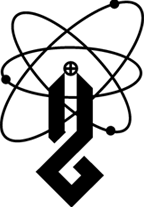
\includegraphics[width=.6cm]{zaeim}
	}
%{\centering
%	بسمه تعالی
%}
\maketitle

\section*{مقدمه}

 این شیوه نامه برای همکاری مشترک بین دانشگاه شریف و دانشکده شهید رضایی در \today تنظیم شده است و هدف آن مشخص کردن روال های سازمانی، اختیارات و اهداف سازمان از این همکاری است. همجنین برنامه ریزی روی نیروی های دانشگاهی، تعریف پروژه برای آن ها و توسعه همکاری های آینده است.


\section{تعاریف}

در این شیوه‌نامه، عنوان های اختصاری زیر، جایگزین عبارت های کامل آن‌ها می‌شود.

\begin{alphabetlist}
	\item\textemf{\textbf{مجموعه}} یا \textemf{\textbf{سازمان}}
	به‌ جای \textemf{مجموعه صنایع الکترونیک زعیم}
	
	\item\textemf{\textbf{دانشگاه}}
	به‌ جای \textemf{دانشگاه صنعتی شریف}
	
	\item\textemf{\textbf{پژوهشکده}}
	به‌ جای \textemf{پژوهشکده شهید رضایی}
	
	\item\textemf{\textbf{امور پژوهشی}}
	به‌جای \textemf{فعالیت های مرتبط با پژوهشکده و یا دانشگاه}
	
	\item\textemf{\textbf{کارگروه فنی}}
	به‌ جای \textemf{کارگروه فنی تعریف و تایید پروژه، تعیین نحوه تحویل و دریافت و  ارزیابی پروژه های تحویلی به پژوهشکده} که ترکیب آن در بند \ref{} ماده \ref{} آورده شده است.

	\item\textemf{\textbf{برون سپاری}}
	به جای \textemf{
	واگذاری تمام یا بخشی از فعالیت های سازمانی	مشخص و قابل واگذاری به بخش امور پژوهشی
}

	\item\textemf{\textbf{خوش تعریف}}
به جای \textemf{پروژه هایی که قابلیت برون سپاری شدن داشته باشند}



	\item\textemf{\textbf{سطح دسترسی}}
به جای \textemf{میزان اختیار بخش امور پژوهشی واجد صلاحیت و افراد مجاز در مورد استفاده از داده ها، سخت افزار}

	
	\item\textemf{\textbf{میزان ریسک پذیری}}
	به جای \textemf{میزان اعتماد سازمانی که برای احقاق اهداف برنامه ریزی پروژه ها، تخصیص داده می‌شود.}
	
	
	\item\textemf{\textbf{کارمزد}}
	به جای \textemf{میزان حق الزحمه‌ای که بابت هر یک از شیوه‌های پروژشی تخصیص داده می‌شود.}


\item\textemf{\textbf{ناظر فنی}}
به جای \textemf{فردی از طرف سازمان که مسئولیت پیگیری پروژه‌های تعریف شده و بررسی عملکرد و روال پیشرفتی را بر عهده دارد.}


\item\textemf{\textbf{رابط سازمان}}
به جای \textemf{فردی از طرف سازمان یا پژوهشکده، که مسيولیت هماهنگی بین اساتید دانشگاه و دانشجویان، ناظر فنی سازمان و پژوهشکده را برعهده دارد.} که در این شیوه نامه، جناب دکتر وثوقی وحدت، عضو هیات علمی دانشگاه شریف و ریاست پژوهشکده شهید رضایی به عنوان رابط سازمان شناخته می‌شود. 


\end{alphabetlist}



\section{تقسیم بندی پروژه‌ها}\label{sec:projects}


تعریف پروژه و جزئیات فنی آن بر عهده کارگروه فنی سازمان است. خروجی های این کارگروه پروژه های خوش تعریف است تا قابلیت برون سپاری داشته باشند.

\begin{note}\label{note:pr-recom}
	پیشنهاد پروژه از خارج سازمان نیز به داخل آن ممکن است و لازم است تا به تاییدیه کارگروه فنی برسد تا قابلیت اجرایی پیدا کند.
\end{note}


\subsection{شرایط پروژه های خوش تعریف}
پروژه های سازمانی برای خوش تعریفی لازم است حائز شرایط زیر باشند. 

\begin{alphabetlist}
	\item
	مسائل امنیتی و درون سازمانی را افشا نکند.
	\item 
	نیازمند پایین ترین سطح دسترسی باشند.
	\item 
	در طول اهداف و مسائل سازمان تعریف شده باشند.
	\item
	حدالمقدور علم محور باشند.
	\item 
	نقطه صفر مشخص داشته باشد.
\end{alphabetlist}

\begin{note}
	مقصود از نقطه صفر، در تعریف خوش تعریفی، این است که راه حلی موجود داشته باشد. خواه این راه حل، موجود در پروژه های متن باز باشد، خواه در پروژه های پیشین مجموعه.
\end{note}





\section{شیوه همکاری های مشترک}

به طور کلی سه شیوه همکاری مشترک قابل تصویر است. هر یک از این شیوه‌ها میزان ریسک پذیری مختلفی دارند و میزان کارمزد مختلفی را می‌توان برایشان درنظر گرفت. هدف این دسته بندی، کاهش هزینه ها و سطح ریسک پذیری و افزایش تعداد نیروهای دانش محور است.

\begin{note}
	مفاد تبصره
	\ref{note:pr-recom}
	لازم است تا در قالب یک یا چند روش از این سه شیوه همکاری تعریف شوند و خارج این چهارچوب، قابل تعریف نمی‌باشند. 
\end{note}



\subsection{گرنت دانشجویی}
این شیوه پایین ترین سطح ریسک پذیری را دارد. کارمزد این شیوه نسبت به شیوه های دیگر کمتر است و مختص دانشجویان در هر سه مقطع کارشناسی، ارشد و دکتری است. در این حالت، پروژه‌ای طبق ماده
\ref{sec:projects}
به عنوان پروژه درسی یا پروژه کارشناسی، ارشد یا دکتری دانشجو تعریف می‌شود و به تایید کارگروه فنی سازمان می‌رسد. 
در این طرح، علاوه بر دانشجو، لازم است یک استاد به عنوان استاد راهنمای دانشجو شرکت کند.


نحوه گزارش دهی در این نوع فعالیت، به صورت توافقی با ناظر سازمان و استاد راهنما است و لازم است در بازه های معین و مشخص شده، دانشجو روال پیشرفت خود را گزارش می‌دهد. نحوه کار دانشجویان در حالت به صورت دورکاری خواهد بود.

در این شیوه، جناب دکتر وثوقی وحدت، به عنوان رابط سازمان و ریاست پژوهشکده، مسیولیت هماهنگی با اساتید دانشگاه و دانشچویان را بر عهده دارند و به ناظر سازمان در پیشبرد این روش کمک می‌کنند.

\begin{note}
	داوطلبان این روش در صورت تمایل برای فعالیت حضوری، در صورت وجود ظرفیت و موافقت جناب دکتر وثوقی وحدت، در پژوهشکده حاضر شوند.
\end{note}

\begin{note}
	علاقه مندان در حوزه فناوری های همگرا 
	\LTRfootnote{\url{https://www.ee.sharif.edu/convergent-technologies}}
	نیز می‌توانند در گرنت دانشجویی، پروژه های خود را تعریف کنند و از مزایای فناوری های همگرا بهره‌مند شوند.
\end{note}


از مزایای این روش برای داوطلبان، دریافت گرنت مالی، بیمه دانش بنیان و انجام یک پروژه علم محور در راستای اهداف سازمان به عنوان پروژه مقطع تحصیلی شان است. عملکرد دانشجویان در این روش به صورت دقیق بررسی می‌شود و تلاش می‌شود تا حد اکثر بهره برداری از آن فرد شود که در صورت رضایت سازمان از آن فرد، امکان همکاری در سایر روش ها مانند قرارداد یا سربازی برای این افراد میسر خواهد بود.

\subsection{پروژه در قالب امور پژوهشی}
این شیوه می‌تواند کارمزد بالاتری نسبت به گرنت دانشجویی داشته باشد و علاوه بر دانشجویان، فارغ التحصیلان دانشگاه را نیز می‌تواند شامل شود. در این طرح افراد به صورت دورکاری و یا نیمه حضوری در قالب پژوهشکده تحت نظر ناظر سازمان، فعالیت می‌کنند و پیوسته در طی بازه های زمانی مشخص گزارش پیشرفت می‌دهند.

برای تایید این شیوه، لازم از پروژه به تایید کارگروه فنی برسد. شرایط کار در این شیوه، به صورت تمام وقت یا  پاره وقت است و داوطلبان لازم است تا با رابط و ناظر سازمان در ارتباط باشند. 

\begin{note}
	پروژه های تعریف شده در این حالت نیز می‌تواند به کمک یک استاد راهنما در کنار رابط و ناظر سازمان تعریف شوند اما در حالت کلی نیازی به استاد راهنما نیست و تنها لازمه آن ارتباط با رابط و ناظر سازمان است.
\end{note}

مزایای این روش نسبت به روش قبلی برای علاقه مندان، این است که روال پیشرفت و ارتقا در آن سریع تر است. همچنین هزینه آن می‌تواند از گرنت بالاتر باشد و به پروژه ای که انجام داده می‌شود، بستگی دارد. در این شیوه، بیمه دانش بنیان برای متقاضیان رد می‌شود. لذا داوطلبانی که پروژه مقطع تحصیلی خود را انتخاب کرده اند و یا فارغ التحصیل شده اند، برای همکاری با سازمان یا افزایش امتیاز نخبگانی خود، می‌توانند بدین شیوه همکاری داشته باشند.


\subsection{قراردادی}

سطح ریسک پذیری این روش و مقدار کارمزد و دسترسی در بیشترین حالت خود است. افراد به صورت حضوری و نیمه حضوری می‌توانند در این شیوه ثبت درخواست کنند.  از آنجایی که میزان ریسک این حالت، بیشتر است، سازمان نیازمند اعتماد بیشتری به افراد است. این اعتماد از طریق رزومه و فعالیت های قبلی متقاضی یا از طریق دو شیوه قبل حاصل شده است. بیمه در این روش می‌تواند به صورت دانش بنیان و یا ترجیحا سازمانی باشد.
 
 \begin{note}
 	روال پیشرفت در این روش، به صورت سازمانی است که در ماده 
 	\ref{sec:}
 	بدان اشاره شده است.
 \end{note}
 
 
\subsection{سربازی (امریه و پروژه)}

این حالت همکاری، یک همکاری دو طرفه است. از طرف سازمان، پروژه و امریه سربازی میسر است. از طرف پژوهشکده، بیمه دانش بنیانی استفاده می‌شود. بدین ترتیب داوطلبان در این موضوع در صورت کسب امتیاز های امریه، دانش آموختگی و فناور، می‌توانند از تسهیلات این مجموعه استفاده کنند.







\section{دسته بندی افراد}

افراد از لحاظ فنی برای کسب پروژه ها، دسته بندی می‌شوند. دسته بندی ها به شرح زیر خواهد بود.













\section{شرح وظایف کارگروه فنی}

وظیفه اصلی کمیته فنی، تعریف پروژه، نحوه انتقال آن به پژوهشکده و نحوه دریافت آن است. اعضای کمیته فنی شامل ناظر سازمان، مدیر محصول و تیم لید های فنی و ... است. کمیته فنی یک عضو به عنوان مسئول کمیته دارد که وظیفه آن هماهنگی بین اعضای کمیته و نظارت بر انجام فعالیت ها است. کمیته فنی از طریق ناظر فنی با متقاضیان پروژه و رابط سازمان در ارتباط است.

از جمله وظایفی که کمیته فنی در احقاق آن تلاش می‌کند، مسیله‌ی خوش تعریفی و خوش تعریف سازی پروژه هاست. مسایل موجود دو نوع هستند. یا از ابتدا خوش تعریف هستند و یا باید خوش تعریف شوند. خوش تعریف سازی پروژه ها روالی چالشی دارد و برای همین از مسایل مهم در کمیته است.
برای این کار لازم است تا به طور هوشمندانه ای مسئله، یا داده، یا راه حل، تغییر پیدا کند به طوری که شرایط خوش تعریفی برای آن صادق شود.

از دیگر وظایف آن، تهیه استاندارد های سازمانی برای تعریف نحوه تحویل دادن و یا گرفتن پروژه است که منجر به بحث فنی کمیته مربوط است.

از طرف دیگر  در این کمیته با همکاری ناظر سازمان، روند پیشرفت پروژه ها ارزیابی می‌شود. خروجی این ارزیابی نحوه همکاری های آینده با داوطلب را مشخص می‌کند. این همکاری می‌تواند به صورت پروژه‌ای ادامه پیدا کند و تغییر در سطح پروژه مدنظر باشد یا تغییر در سطح حقوقی و یا سطح اعتماد سازمانی.

تایید افراد داوطلب و تعیین دسته فنی آن ها، برعهده کمیته فنی خواهد بود. در این حالت یک نفر به نمایندگی از کارگروه، با افراد داوطلب مصاحبه خواهد کرد و دسته آن را مشخص می‌کند و با همکاری با ناظر سازمان، برای پیشرفت آن فرد و پیشبرد اهداف طرح ریزی شده، برنامه ریزی می‌کنند.

همچنین این که کدام دسته پروژه و نوع همکاری به کدام دسته افراد تعلق گیرد، برعهده تصمیم کمیته فنی خواهد بود.








































\end{document}






